\documentclass[12pt]{article}
\usepackage{setspace}  % To use linespacing
\usepackage{indentfirst} % Indents first line after sections
\usepackage{amssymb} % For \mathbb
\usepackage{enumerate} % For changing labels of enumerate
\usepackage[margin=1in]{geometry} % For editing margins
\usepackage{tikz} % Tikz drawing for graphs
\usetikzlibrary{arrows.meta} % Allows customizing arrows
\usetikzlibrary{backgrounds} % For framing a tikzpicture
\usepackage{amsmath}

% Make new commands
\newcommand{\N}{\mathbb{N}}
\newcommand{\R}{\mathbb{R}}
\newcommand{\Z}{\mathbb{Z}}
\newcommand{\abs}[1]{\left|#1\right|}
\newcommand{\paren}[1]{\left(#1\right)}
\newcommand{\fivespace}{\space\space\space\space\space}

% Start main document
\begin{document}
\onehalfspacing
\hfill Frank Cline

\hfill Math 307

\hfill HW 6

% Sections
% 6.1 # 8, 10, 13a, 14b, 15, 16, 20
% 6.2 # 2, 7, 8, 15

% SECTION 6.1 # 8, 10, 13a, 14b, 15, 16, 20
\section*{6.1}
\begin{enumerate}

\setcounter{enumi}{7}
% 8
\item Can a graph have an odd number of vertices of odd degree? Explain.
	
	No.

\setcounter{enumi}{9}
% 10
\item Draw a picture of the graph $G$ with $V(G)=\{x,y,z,w\},E(G)=\{a,b,c,d,f,g,h\}$ and $\gamma$ as given by the table\\
\begin{tabular}{c|c c c c c c c}
	$e$ & $a$ & $b$ & $c$ & $d$ & $f$& $g$ & $h$\\
	\hline
	\\
	$\gamma(e)$ & $\{x,y\}$ & $\{x,y\}$ & $\{w,x\}$ & $\{w,y\}$ & $\{y,z\}$ & $\{y,z\}$ & $\{w,z\}$\\
\end{tabular}
\[
	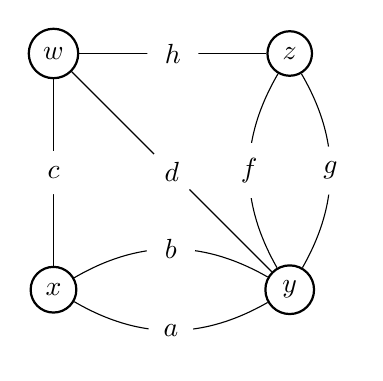
\begin{tikzpicture}
	\begin{scope}[every node/.style={circle,thick,draw}]
	    	\node (x) at (0,0) {$x$};
	    	\node (y) at (3,0) {$y$};
	    	\node (w) at (0,3) {$w$};
		\node (z) at (3,3) {$z$};
	\end{scope}
	
	\begin{scope}[>={Stealth[black]},
	              every node/.style={fill=white,circle},
	              every edge/.style={draw=black}]
		\path (x) edge[bend right = 30] node {$a$} (y);
		\path (x) edge[bend left = 30] node {$b$} (y);
		\path (w) edge node {$c$} (x);
		\path (w) edge node {$d$} (y);
		\path (y) edge[bend left = 30] node {$f$} (z);
		\path (y) edge[bend right = 30] node {$g$} (z);		
		\path (w) edge node {$h$} (z);
	\end{scope}
	\end{tikzpicture}
\]

\setcounter{enumi}{12}
% 13a
\item
	\begin{enumerate}
	\item Draw pictures of all five of the regular graphs that have four vertices each vertex of degree 2. "All" here means
	that every regular graph with four vertices and each vertex of degree 2 is isomorphic to one of the five, and no two
	of the five are isomorphic to each other.
	\end{enumerate}

	\[
	% Graph 1 & 2
	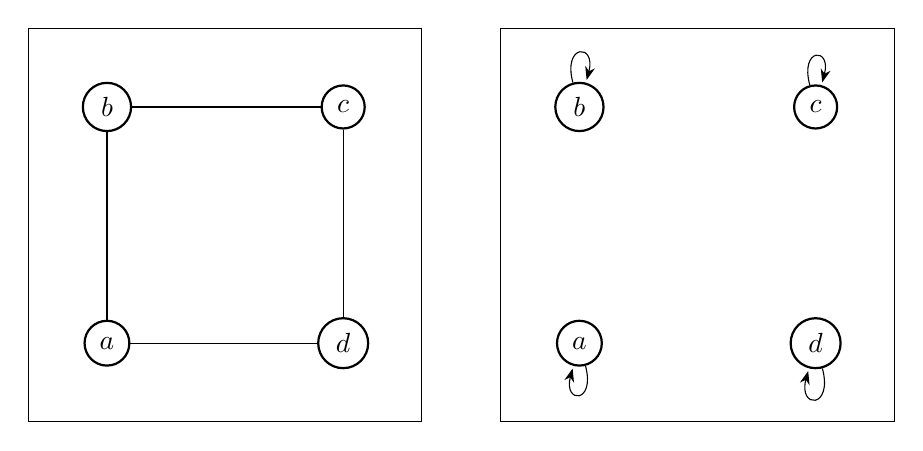
\begin{tikzpicture}
	\draw (-1,-1) rectangle (4,4);
	\draw (5,-1) rectangle (10,4);
	\begin{scope}[every node/.style={circle,thick,draw}]
	    	\node (1) at (0,0) {$a$};
	    	\node (2) at (0,3) {$b$};
	    	\node (3) at (3,3) {$c$};
		\node (4) at (3,0) {$d$};
	    	\node (5) at (6,0) {$a$};
	    	\node (6) at (6,3) {$b$};
	    	\node (7) at (9,3) {$c$};
		\node (8) at (9,0) {$d$};
	\end{scope}
	
	\begin{scope}[>={Stealth[black]},
	              every node/.style={fill=white,circle},
	              every edge/.style={draw=black}]
		\path (1) edge (2);
		\path (2) edge (3);
		\path (3) edge (4);
		\path (4) edge (1);
		\path (5) edge[loop below] (5);
		\path (6) edge[loop above] (6);
		\path (7) edge[loop above] (7);
		\path (8) edge[loop below] (8);
	\end{scope}
	\end{tikzpicture}
	\]
	\[
	% Graph 3 & 4
	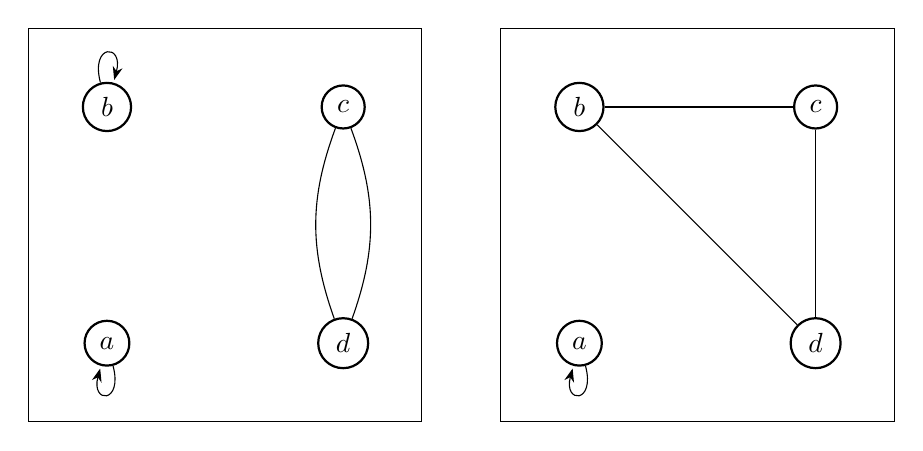
\begin{tikzpicture}
	\draw (-1,-1) rectangle (4,4);
	\draw (5,-1) rectangle (10,4);
	\begin{scope}[every node/.style={circle,thick,draw}]
	    	\node (9) at (0,0) {$a$};
	    	\node (10) at (0,3) {$b$};
	    	\node (11) at (3,3) {$c$};
		\node (12) at (3,0) {$d$};
	    	\node (13) at (6,0) {$a$};
	    	\node (14) at (6,3) {$b$};
	    	\node (15) at (9,3) {$c$};
		\node (16) at (9,0) {$d$};
	\end{scope}
	
	\begin{scope}[>={Stealth[black]},
	              every node/.style={fill=white,circle},
	              every edge/.style={draw=black}]
		\path (9) edge[loop below] (9);
		\path (10) edge[loop above] (10);
		\path (11) edge[bend left=20] (12);
		\path (11) edge[bend right=20] (12);
		\path (13) edge[loop below] (13);
		\path (14) edge (15);
		\path (15) edge (16);
		\path (16) edge (14);
	\end{scope}
	\end{tikzpicture}
	\]
	\[
	% Graph 5
	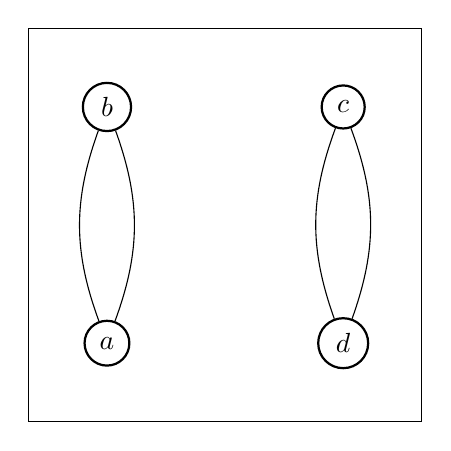
\begin{tikzpicture}
	\draw (-1,-1) rectangle (4,4);
	\begin{scope}[every node/.style={circle,thick,draw}]
	    	\node (17) at (0,0) {$a$};
	    	\node (18) at (0,3) {$b$};
	    	\node (19) at (3,3) {$c$};
		\node (20) at (3,0) {$d$};
	\end{scope}
	
	\begin{scope}[>={Stealth[black]},
	              every node/.style={fill=white,circle},
	              every edge/.style={draw=black}]
		\path (17) edge[bend right=20] (18);
		\path (17) edge[bend left=20] (18);
		\path (19) edge[bend right=20] (20);
		\path (19) edge[bend left=20] (20);
	\end{scope}
	\end{tikzpicture}
	\]

% 14b
\item
	\begin{enumerate}
	\setcounter{enumii}{1}
	\item Draw pictures of the two graphs with four vertices and four edges that have no loops or parallel edges.
	\end{enumerate}

	\[
	% Graph 1 & 2
	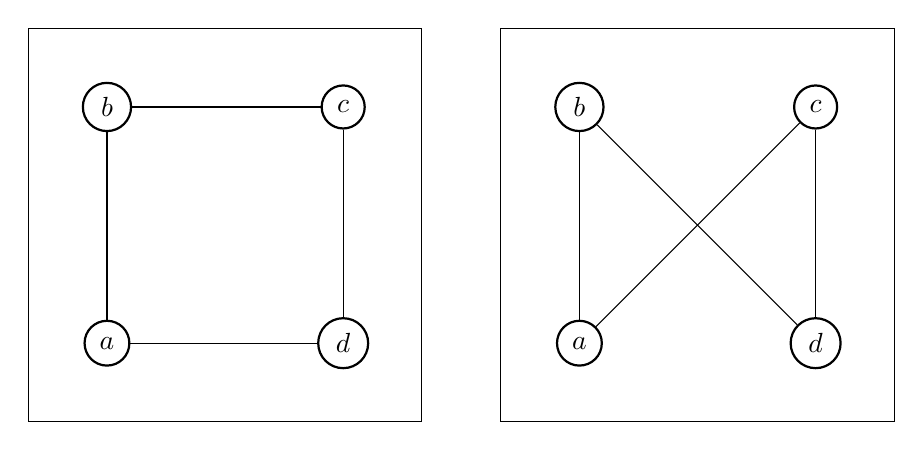
\begin{tikzpicture}
	\draw (-1,-1) rectangle (4,4);
	\draw (5,-1) rectangle (10,4);
	\begin{scope}[every node/.style={circle,thick,draw}]
	    	\node (1) at (0,0) {$a$};
	    	\node (2) at (0,3) {$b$};
	    	\node (3) at (3,3) {$c$};
		\node (4) at (3,0) {$d$};
	    	\node (5) at (6,0) {$a$};
	    	\node (6) at (6,3) {$b$};
	    	\node (7) at (9,3) {$c$};
		\node (8) at (9,0) {$d$};
	\end{scope}
	
	\begin{scope}[>={Stealth[black]},
	              every node/.style={fill=white,circle},
	              every edge/.style={draw=black}]
		\path (1) edge (2);
		\path (2) edge (3);
		\path (3) edge (4);
		\path (4) edge (1);
		\path (5) edge (7);
		\path (6) edge (8);
		\path (5) edge (6);
		\path (7) edge (8);
	\end{scope}
	\end{tikzpicture}
	\]

% 15
\item Which, if any, of the pairs of graphs shown are isomorphic? Justify your answer by describing an isomorphism or explaining why one does not exist.
	\begin{enumerate}
	\item .\\
		% Graph a
		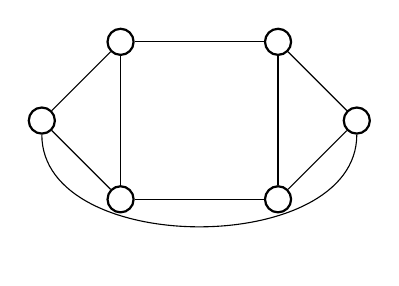
\begin{tikzpicture}
		\begin{scope}[every node/.style={circle,thick,draw}]
		    	\node (1) at (0,0) {};
			\node (2) at (2,0) {};
		    	\node (3) at (3,1) {};
			\node (4) at (2,2) {};
		    	\node (5) at (0,2) {};
			\node (6) at (-1,1) {};			
		\end{scope}
		
		\begin{scope}[>={Stealth[black]},
		              every node/.style={fill=white,circle},
		              every edge/.style={draw=black}]
			\path (1) edge (2);
			\path (1) edge (5);
			\path (1) edge (6);
			\path (2) edge (3);
			\path (2) edge (4);
			\path (3) edge (4);
			\path (3) edge[bend left=90] (6);
			\path (4) edge (5);
			\path (5) edge (6);
		\end{scope}
		\end{tikzpicture}
	\item .\\
		% Graph b
		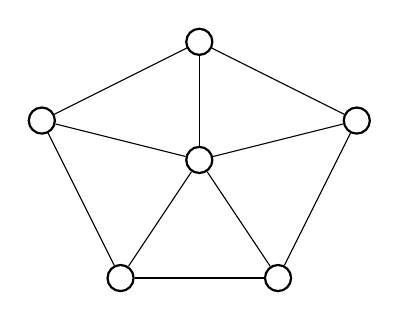
\begin{tikzpicture}
		\begin{scope}[every node/.style={circle,thick,draw}]
		    	\node (1) at (0,0) {};
			\node (2) at (2,0) {};
		    	\node (3) at (3,2) {};
			\node (4) at (1,3) {};
		    	\node (5) at (-1,2) {};
			\node (6) at (1,1.5) {};			
		\end{scope}
		
		\begin{scope}[>={Stealth[black]},
		              every node/.style={fill=white,circle},
		              every edge/.style={draw=black}]
			\path (1) edge (2);
			\path (2) edge (3);
			\path (3) edge (4);
			\path (4) edge (5);
			\path (5) edge (1);
			\path (6) edge (1);
			\path (6) edge (2);
			\path (6) edge (3);
			\path (6) edge (4);
			\path (6) edge (5);
		\end{scope}
		\end{tikzpicture}
	\item .\\
		% Graph c
		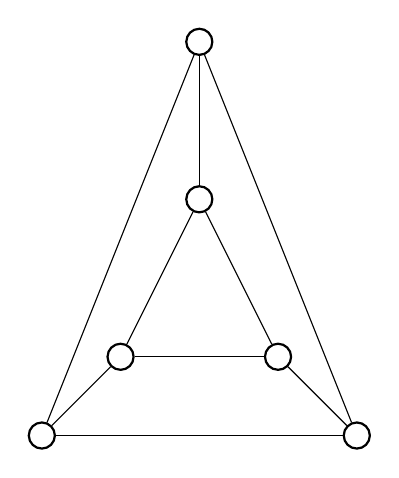
\begin{tikzpicture}
		\begin{scope}[every node/.style={circle,thick,draw}]
		    	\node (1) at (0,0) {};
			\node (2) at (4,0) {};
		    	\node (3) at (2,5) {};
			\node (4) at (1,1) {};
		    	\node (5) at (3,1) {};
			\node (6) at (2,3) {};			
		\end{scope}
		
		\begin{scope}[>={Stealth[black]},
		              every node/.style={fill=white,circle},
		              every edge/.style={draw=black}]
			\path (1) edge (2);
			\path (2) edge (3);
			\path (3) edge (1);
			\path (4) edge (5);
			\path (5) edge (6);
			\path (6) edge (4);
			\path (1) edge (4);
			\path (2) edge (5);
			\path (3) edge (6);
		\end{scope}
		\end{tikzpicture}
	\item .\\
		% Graph d
		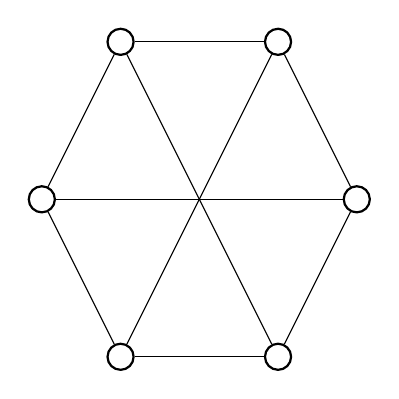
\begin{tikzpicture}
		\begin{scope}[every node/.style={circle,thick,draw}]
		    	\node (1) at (0,0) {};
			\node (2) at (2,0) {};
		    	\node (3) at (3,2) {};
			\node (4) at (2,4) {};
		    	\node (5) at (0,4) {};
			\node (6) at (-1,2) {};			
		\end{scope}
		
		\begin{scope}[>={Stealth[black]},
		              every node/.style={fill=white,circle},
		              every edge/.style={draw=black}]
			\path (1) edge (2);
			\path (2) edge (3);
			\path (3) edge (4);
			\path (4) edge (5);
			\path (5) edge (6);
			\path (6) edge (1);
			\path (1) edge (4);
			\path (2) edge (5);
			\path (3) edge (6);
		\end{scope}
		\end{tikzpicture}

	% Answer to 15
	(a $\not\cong$ b) Not isomorphic because the maximum degree of a vertex in $a$ is 3, while the maximum degree of a vertex 
	in $b$ is 5. \\
	(a $\cong$ c) Isomorphic by labeling each graph:\\
		% Graph a
		\[
		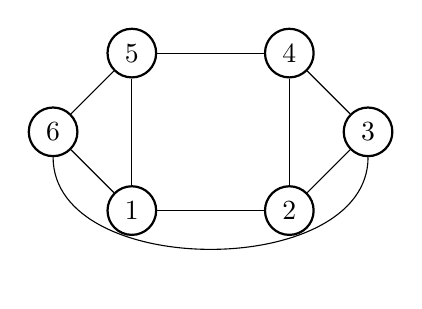
\begin{tikzpicture}
		\begin{scope}[every node/.style={circle,thick,draw}]
		    	\node (1) at (0,0) {$1$};
			\node (2) at (2,0) {$2$};
		    	\node (3) at (3,1) {$3$};
			\node (4) at (2,2) {$4$};
		    	\node (5) at (0,2) {$5$};
			\node (6) at (-1,1) {$6$};			
		\end{scope}
		
		\begin{scope}[>={Stealth[black]},
		              every node/.style={fill=white,circle},
		              every edge/.style={draw=black}]
			\path (1) edge (2);
			\path (1) edge (5);
			\path (1) edge (6);
			\path (2) edge (3);
			\path (2) edge (4);
			\path (3) edge (4);
			\path (3) edge[bend left=90] (6);
			\path (4) edge (5);
			\path (5) edge (6);
		\end{scope}
		\end{tikzpicture}
		% Graph c
		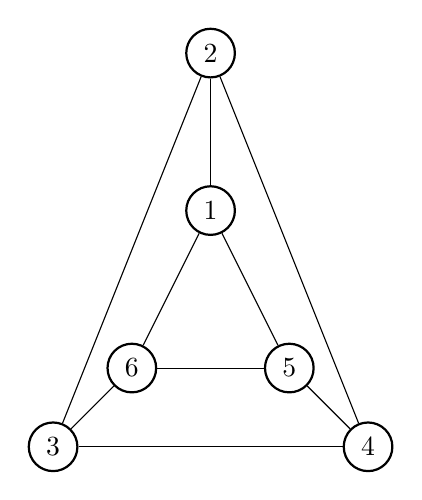
\begin{tikzpicture}
		\begin{scope}[every node/.style={circle,thick,draw}]
		    	\node (1) at (0,0) {$3$};
			\node (2) at (4,0) {$4$};
		    	\node (3) at (2,5) {$2$};
			\node (4) at (1,1) {$6$};
		    	\node (5) at (3,1) {$5$};
			\node (6) at (2,3) {$1$};			
		\end{scope}
		
		\begin{scope}[>={Stealth[black]},
		              every node/.style={fill=white,circle},
		              every edge/.style={draw=black}]
			\path (1) edge (2);
			\path (2) edge (3);
			\path (3) edge (1);
			\path (4) edge (5);
			\path (5) edge (6);
			\path (6) edge (4);
			\path (1) edge (4);
			\path (2) edge (5);
			\path (3) edge (6);
		\end{scope}
		\end{tikzpicture}
		\]
	(a $\not\cong$ d) Not isomorphic because $a$ has a cycle of length 3 while $d$ does not.\\
	(b $\not\cong$ c) Not isomorphic because the maximum degree of a vertex in $c$ is 3, while the maximum degree of a vertex 
	in $b$ is 5. \\
	(b $\not\cong$ d) Not isomorphic because the maximum degree of a vertex in $d$ is 3, while the maximum degree of a vertex 
	in $b$ is 5. \\
	(c $\not\cong$ d) Not Isomorphic because $c$ has a cycle of length 3 while $d$ does not.
	\end{enumerate}

% 16
\item Describe an isomorphism between the graphs:
\[
% Graph 1 & 2
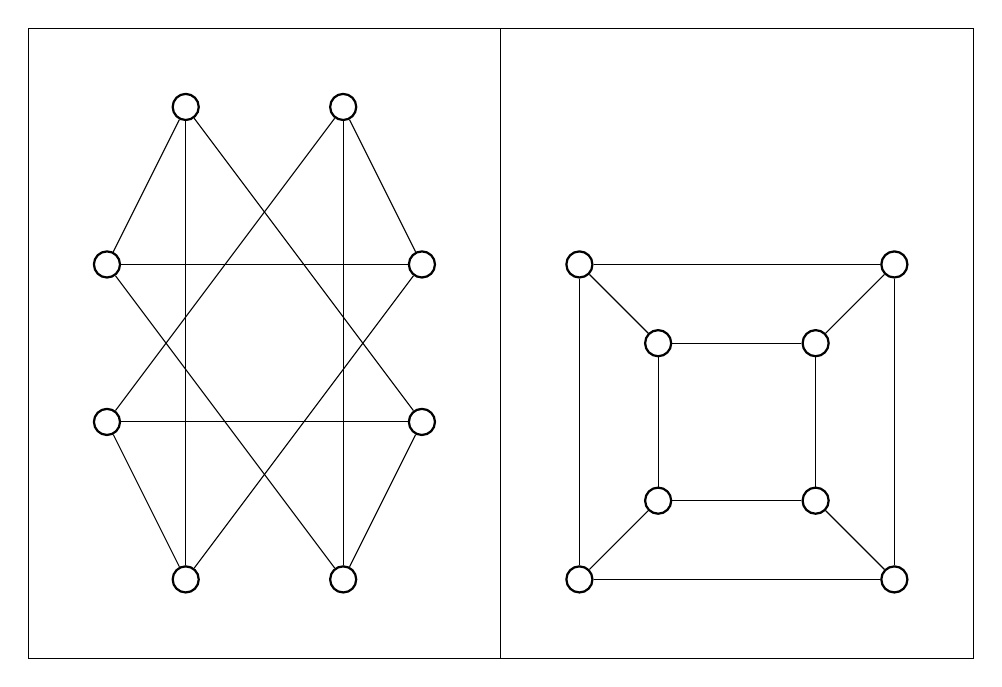
\begin{tikzpicture}
\draw (-2,-1) rectangle (4,7);
\draw (4,-1) rectangle (10,7);
\begin{scope}[every node/.style={circle,thick,draw}]
    	\node (1) at (0,0) {};
    	\node (2) at (2,0) {};
    	\node (3) at (3,2) {};
	\node (4) at (3,4) {};
    	\node (5) at (2,6) {};
    	\node (6) at (0,6) {};
    	\node (7) at (-1,4) {};
	\node (8) at (-1,2) {};

    	\node (11) at (5,0) {};
    	\node (12) at (9,0) {};
    	\node (13) at (9,4) {};
	\node (14) at (5,4) {};
    	\node (15) at (6,1) {};
    	\node (16) at (8,1) {};
    	\node (17) at (8,3) {};
	\node (18) at (6,3) {};
\end{scope}

\begin{scope}[>={Stealth[black]},
              every node/.style={fill=white,circle},
              every edge/.style={draw=black}]
	\path (1) edge (4);
	\path (1) edge (8);
	\path (1) edge (6);
	\path (2) edge (7);
	\path (2) edge (5);
	\path (2) edge (3);
	\path (3) edge (8);
	\path (3) edge (6);
	\path (4) edge (7);
	\path (4) edge (5);
	\path (5) edge (8);
	\path (6) edge (7);

	\path (11) edge (14);
	\path (11) edge (15);
	\path (11) edge (12);
	\path (12) edge (16);
	\path (12) edge (13);
	\path (13) edge (17);
	\path (13) edge (14);
	\path (14) edge (18);
	\path (15) edge (16);
	\path (15) edge (18);
	\path (16) edge (17);
	\path (17) edge (18);
\end{scope}
\end{tikzpicture}
\]
% Answer to 16
	\[
	% Graph 1 & 2
	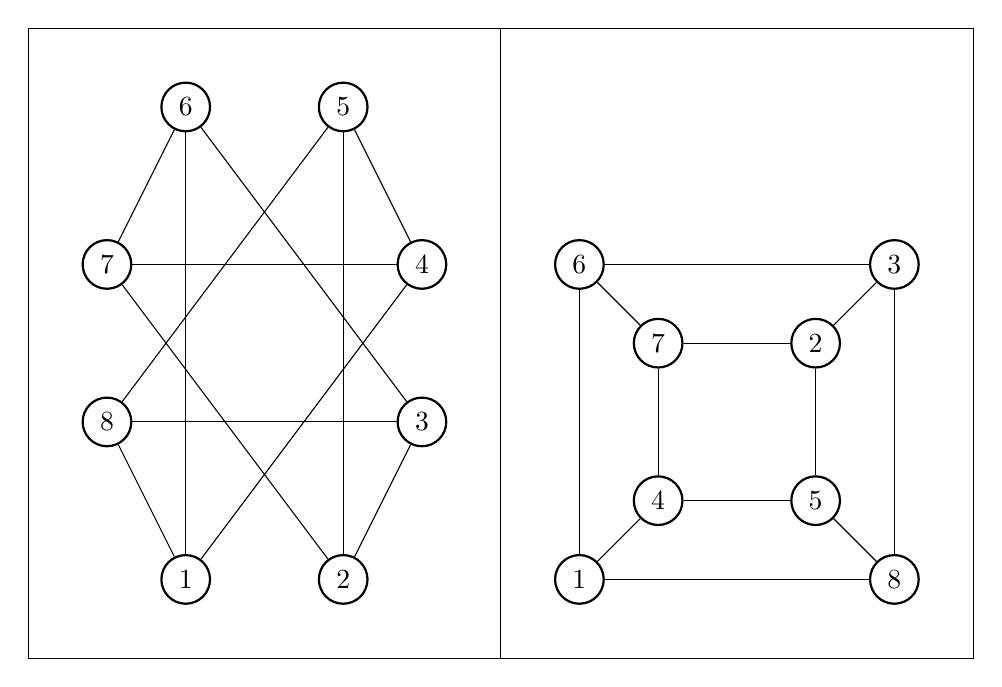
\begin{tikzpicture}
	\draw (-2,-1) rectangle (4,7);
	\draw (4,-1) rectangle (10,7);
	\begin{scope}[every node/.style={circle,thick,draw}]
	    	\node (1) at (0,0) {$1$};
	    	\node (2) at (2,0) {$2$};
	    	\node (3) at (3,2) {$3$};
		\node (4) at (3,4) {$4$};
	    	\node (5) at (2,6) {$5$};
	    	\node (6) at (0,6) {$6$};
	    	\node (7) at (-1,4) {$7$};
		\node (8) at (-1,2) {$8$};
	
	    	\node (11) at (5,0) {$1$};
	    	\node (12) at (9,0) {$8$};
	    	\node (13) at (9,4) {$3$};
		\node (14) at (5,4) {$6$};
	    	\node (15) at (6,1) {$4$};
	    	\node (16) at (8,1) {$5$};
	    	\node (17) at (8,3) {$2$};
		\node (18) at (6,3) {$7$};
	\end{scope}
	
	\begin{scope}[>={Stealth[black]},
	              every node/.style={fill=white,circle},
	              every edge/.style={draw=black}]
		\path (1) edge (4);
		\path (1) edge (8);
		\path (1) edge (6);
		\path (2) edge (7);
		\path (2) edge (5);
		\path (2) edge (3);
		\path (3) edge (8);
		\path (3) edge (6);
		\path (4) edge (7);
		\path (4) edge (5);
		\path (5) edge (8);
		\path (6) edge (7);
	
		\path (11) edge (14);
		\path (11) edge (15);
		\path (11) edge (12);
		\path (12) edge (16);
		\path (12) edge (13);
		\path (13) edge (17);
		\path (13) edge (14);
		\path (14) edge (18);
		\path (15) edge (16);
		\path (15) edge (18);
		\path (16) edge (17);
		\path (17) edge (18);
	\end{scope}
	\end{tikzpicture}
	\]

\setcounter{enumi}{19}
% 20
\item 
	\begin{enumerate}
	% 20a
	\item A graph with 21 edges has seven vertices of degree 1, three of degree 2, seven of degree 3 and the rest of degree 4. 
	How many vertices does it have?\\
		$2\cdot |E(G)|$ = The sum of the degree of all $v\in V(G)$.\\
		$2\cdot 21 = 7(1)+3(2)+7(3)+x(4)=7+6+21+4x=34+4x$\\
		$4x=42-34=8$, so $x=2$.\\
		$7+3+7+2=19$ vertices.
	% 20b
	\item How would your answer to part (a) change if the graph also had six vertices of degree 0?\\
		The answer would include 6 extra vertices, so it would be 25 not 19 vertices.
	\end{enumerate}


\end{enumerate}

\end{document}